% !TEX root = mainthesis.tex
%Chapter 7

\renewcommand{\thechapter}{7}

\chapter{Topological order in quantum systems}
\label{ch:Topology}

Topological order can be found in a wide range of physical systems, from crystalline solids\cite{hasan_colloquium:_2010}, photonic meta-materials\cite{ozawa_topological_2019} and even atmospheric waves\cite{delplace_topological_2017} to optomechanic\cite{peano_topological_2015}, acoustic\cite{yang_topological_2015} and atomic systems\cite{cooper_topological_2019}. Topological systems are a robust foundation for creating quantized channels for transporting electrical current, light, and atmospheric disturbances. These topological effects can be quantified in terms of integer-valued invariants such as the Chern number, applicable to the quantum Hall effect\cite{thouless_quantized_1982,haldane_model_1988}, or the $\mathbb{Z}_2$ invariant suitable for topological insulators\cite{kane_$z_2$_2005}. 

The topology of Bloch bands defines integers that serve to both classify crystalline materials and precisely specify properties, such as conductivity, that are independent of small changes to lattice parameters\cite{hasan_colloquium:_2010}. Topologically non-trivial materials first found application in metrology with the definition of the von Klitzing constant as a standard of resistance, which is now applied in the realization of the kilogram\cite{newell_codata_2018}. Today, topological systems have found applications in the engineering of low loss optical waveguides\cite{ozawa_topological_2019} and present a promising path to quantum computation\cite{nayak_non-abelian_2008}.

We got interested in topology when working on engineering Rashba~\cite{bychkov_oscillatory_1984} type spin-orbit coupling in the lab. Our system had non-trivial topology but it broke from the usual mold of topological materials as it didn't have an underlying crystalline structure that conventionally yields to integer Chern numbers. 

Before describing our experiments that characterize the unconventional topology of a Rashba spin-orbit coupled gas, in this Chapter I take a step back to describe the basic concepts of topology and its applications to the band theory of solids. The ideas of topology and how exactly one can connect donuts with band structures might feel a bit obscure and complicated for non-experts in the field. I wrote this Chapter with that in mind, with the hope that it can be followed by non-experts and provide some insight and intuition about this field. The concepts introduced in this Chapter will be necessary for understanding the results presented in Chapter~\ref{ch:Rashba}.
 
\section{Topology in mathematics} 

Topology is a branch of mathematics that studies continuity~\cite{differential_topology_and_geometry}. The most familiar example might be that of objects being continuously deformed into one another. For example, a donut can be continuously deformed into a coffee mug but if we want to deform it into a pretzel we need to poke more holes in it. This gives us some intuition that the donut and the mug must share the same topology, which is different from that of the pretzel. Topology also studies more abstract objects but I will limit the discussion to closed two-dimensional surfaces in three dimensions, which will be enough to provide some intuition when we define topological invariants for band structures in the following sections.  

The topology of 2D surfaces can be classified by the Euler characteristic, and it is related to the local Gaussian curvature of a surface by the Gauss-Bonet theorem. The Gaussian curvature can be interpreted in the following way: at any point in a surface we can find a normal vector which is orthogonal to the tangent plane of the surface. We can then define a family of planes containing the normal vector and their intersection with the surface defines a family of curves. The curvature of a any of these curves at the point where the planes intersect, which is equal to the quadratic coefficient in a Taylor expansion around that point, is called the normal curvature $\kappa$. When we consider all the normal curvatures, the minimum and maximum of these are called the principal curvatures and are used to define the Gaussian curvature at any point of a surface $K=\kappa_{min}\kappa_{max}$~\cite{differential_topology_and_geometry} 

The Gauss-Bonnet theorem states that the integral of the local Gaussian curvature over the whole surface is equal to the integer valued Euler characteristic
%
\begin{equation}
	\chi = \frac{1}{2\pi}\int_S K dA,
	\label{eq:euler_characteristic}
\end{equation}
%
which is related to the genus $g$ (number of holes or handles in the surface) by $\chi=2(1-g)$. The Gauss-Bonnet theorem is a very powerful result as it relates the local properties of a surface,the Gaussian curvature, with a global topological invariant, the Euler characteristic. \note{Add picture to describe principal curvatures?}

In the following sections I will introduce topological invariants in the context of condensed matter physics, which even though might seem a bit more abstract, their interpretation can be closely related to the concepts just defined in this section. 
\section{Topological order in condensed matter}

Just like topology classifies properties of geometric objects, one important task of condensed matter physics has been to classify phases of matter. Many of these phases, for example magnetic or conducting phases, can be described in terms of order parameters related to spontaneously broken symmetries~\cite{landau_theory_1936}. However, in the past few decades and increasing number of systems have been found where it is only possible to understand their phases and properties in terms of the underlying topology of their quantum states. This new paradigm of physics has been so important that in 2016 the Nobel prize in physics was awarded to David J. Thoules, F. Duncan M. Haldane and J. Michael Kosterlitz for the theoretical discoveries of topological phase transitions and topological phases of matter 

The effects of topology in condensed matter systems were first observed when von Klitzing and colleagues~\cite{klitzing_new_1980} measured the quantized Hall resistance in two-dimensional electron gases subjected to a strong perpendicular magnetic field. The effect can be understood semi-classically by thinking of the electrons' quantized cyclotron orbits\footnote{This is an intuitive but not very complete explanation of the quantum Hall effect, see \cite{tong_lectures_2016} if you want to learn more about this subject.} that give rise to Landau levels. If the Landau levels are filled then there is an energy gap separating two consecutive levels and the material acts as an insulator but if an electric field is applied the orbits drift and the electrons will be `skipping orbits' in the edge as can be seen in Figure~\ref{fig:quantum_hall}, giving rise to what is known as edge states.
% 
\begin{figure*}[htb]
\begin{center}
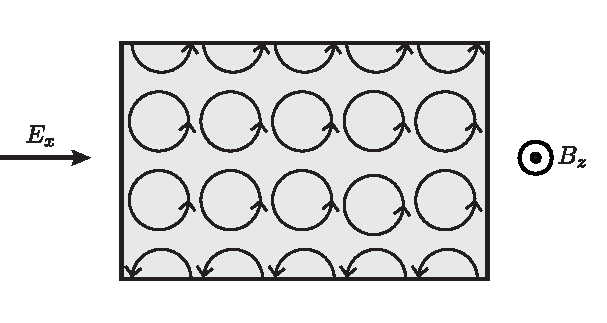
\includegraphics[]{Figures/Chapter7/quantum_hall.pdf}
\caption[The quantum Hall effect]{The quantum Hall effect. An electron gas is confined in a two-dimensional material and a strong magnetic field is applied perpendicular to the plane. The electrons on the bulk travel in cyclotron orbits while the electrons on the edge travel `skipping orbits'.}
\label{fig:quantum_hall}
\end{center}
\end{figure*}

In a seminal paper Thoules, Kohomoto, Nightingale, and den Nijs~\cite{thouless_quantized_1982} explained that the quantization of the Hall conductivity is determined by the underlying topology of the band structure. Just like the Euler characteristic defined in Equation~\ref{eq:euler_characteristic} classifies 2D solids that can be continuously deformed without opening or closing holes, there is a topological invariant that classifies band structures that can be deformed into one another without opening or closing an energy gap. This invariant, initially known as the `TKNN invariant', was later recognized by the mathematical physicist Bary Simon as the `first Chern class invariant from $U(1)$ fiber bundles'~\cite{simon_holonomy_1983}\footnote{See~\cite{geometry_topology_physics} if you want to dive into hardcore topology.} and the TKNN invariant became what is known today as the Chern number or Chern invariant. Another very valuable contribution from Simon's work was that he made the connection between the Chern number and the the Berry's geometrical phase~\cite{berry_michael_victor_quantal_1984} which will be defined in the following sections and will allow us to make a physical interpretation of this otherwise abstract seeming topological invariant. 

\section{Berry phase and Berry curvature}
\label{sec:Berry phase and curvature}

A Berry or geometric phase is used to describe the phase acquired by a quantum state as it moves through a closed trajectory in parameter space. It plays a key role in topological band theory and can help provide a physical interpretation of the Chern number. 

Consider a Hamiltonian $\hat H$ that depends on a set of parameters $\r=(r_1, r_2, ...)$. If the parameters are slowly changed in time, the corresponding change in the system can be described by a path in parameter space $\r(t)$. The state $\ket{\psi(t)}$ evolves according to the time dependent Sch\"odinger equation and at any given time $t$ there is a basis that satisfies
%
\begin{equation}
	\hat H(\r)\ket{n(\r)}=E_n(\r)\ket{n(\r)}
	\label{eq:hamiltonian_eigenvectors}
\end{equation}
%
for $\r=\r(t)$. Suppose the system is initially in state $\ket{n(\r(t=0))}$, if the parameters are changed slowly such that the adiabatic theorem is valid, then at time $t$ the state of the system can be written as
%
\begin{equation}
	\ket{\psi(t)}=\exp\Big\{-\frac{i}{\hbar}\int_0^tdt'E_n(\r(t'))\Big\}\exp(i\gamma_n(t))\ket{n(\r(t))},
	\label{eq:berry_wf}
\end{equation}
%
where the first exponential term corresponds to a dynamical phase factor, and the second term is a geometric phase. By imposing that $\ket{\psi(t)}$ satisfies the time-dependent Schr\"odinger equation one finds that 
%
\begin{equation}
	\gamma_n(t)=i\braket{n(\r)}{\nabla_{\r}n(\r)}\cdot\dot{\r}(t),
\end{equation}
%
where the term
%
\begin{equation}
	\mathbf{A}_n(\r)=i\braket{n(\r)}{\nabla_{\r}n(\r)}
	\label{eq:berry_connection}
\end{equation}
%
 is usually referred to as the Berry connection\footnote{This is related to the connection defined in differential geometry that is used to describe things like parallel transport.} or the Berry vector potential for reasons that will become apparent. Because eigenvectors can only be defined up to a global phase, $\mathbf{A}$ is a gauge dependent quantity. If we make a gauge transformation such that $\ket{n(\k)}\rightarrow\e^{i\xi(\k)}\ket{n(\k)}$ then the Berry connection is also transformed as $\mathbf{A}_n(\k)\rightarrow\mathbf{A}_n(\k)-\nabla_{\k}\xi(\k)$. However if we integrate the Berry connection on a closed loop
%
\begin{equation}
	\gamma_n(\mathcal{C})=\oint_{\mathcal{C}} \mathbf{A}_n(\r)\cdot d\mathbf{l},
	\label{eq:berry_phase}
\end{equation}
%
we obtain the Berry phase which, unlike the Berry connection, is gauge independent (modulo $2\pi$). %It should also be noted that  $\gamma_n$ only depends on the geometry of the path and is independent of how it was traversed in time.

An alternative way to compute Berry's phase uses Stokes's theorem from vector calculus
%
\begin{align}
	\oint_{\mathcal{C}} \mathbf{A}_n\cdot d\mathbf{l}=&\int_{\mathcal{S}}\nabla\times\mathbf{A}_n\cdot d\mathbf{S} \nonumber \\
	=& \int_{\mathcal{S}}\mathbf{\Omega}_n\cdot d\mathbf{S},
	\label{eq:berry_connection}
\end{align}
%
where the vector field $\mathbf{\Omega}_n=\nabla\times\mathbf{A}_n$ is known as the Berry curvature or Berry fieldT. By rewriting the Berry phase in this way, its resemblance with the definition of the Euler characteristic from Equation~\ref{eq:euler_characteristic} becomes apparent.

Using some vector calculus identities the Berry curvature can be rewritten as

\begin{align}
	\mathbf{\Omega}_n=&i[\nabla_{\r}\bra{n}]\times[\nabla_{\r}\ket{n}]\nonumber \\ 
	=& \sum_{j\neq n} i[\bra{n}\nabla_{\r}\ket{j}]\times[\bra{j}\nabla_{\r}\ket{n}] \nonumber \\
	=& i\sum_{j\neq n}\frac{\bra{n}\nabla_{\r}\hat{H}\ket{j}\times\bra{j}\nabla_{\r}\hat{H}\ket{n}}{(E_j-E_n)^2},
	\label{eq:alternative_berry_con}
\end{align}
%
where $\bra{n}\nabla_{\r}\ket{j}$ was replaced with $\bra{n}\nabla_{\r}\hat{H}\ket{j}/(E_j-E_n)$ by differentiating Equation~\ref{eq:hamiltonian_eigenvectors}. This expression shows that $\mathbf{\Omega}_n$ is a gauge independent quantity as it does not depend on the derivatives of a particular gauge choice for $\ket{n}$ but rather on $\nabla_{\r}\hat{H}$ which is gauge independent. Also we can see that $\mathbf{\Omega}_n$ becomes singular when there are degeneracies present in the Hamiltonian, and these degeneracies act as `sources' for the Berry connection. Finally, even though the system may remain in state $\ket{n}$ during the adiabatic evolution, this expression for the Berry curvature makes it explicit that other eigenstates of the Hamiltonian have an influence in the Berry phase acquired. 

\subsection{Aharonov-Bohm phase as an example of a Berry's phase}

A familiar example of geometric phases is the Aharonov-Bohm phase~\cite{aharonov_significance_1959} gained by an electrons moving along closed trajectories around a solenoid. This phase was initially conceived as a way of showing that in quantum mechanics magnetic vector potentials, typically conceived only as mathematical objects, can have a physical effect on the wave function. They considered a coherent electron beam split into two paths around a solenoid that produces a magnetic field $\mathbf{B}$ as shown in Figure~\ref{fig:aharonov_bohm}. Outside the solenoid the magnetic field $\mathbf{B}=0$, but there can be a non-zero magnetic vector potential such that $\mathbf{B}=\nabla\times\mathbf{A}$. The two beams are later recombined. Even though the electron's trajectories are not modified, when looking at the interference pattern one finds that the two paths acquired different phases, and their difference is remarkably equal to magnetic flux piercing the area enclosed by the electrons path $\Delta\varphi = 2\pi \Phi_B/\Phi_0$, where $\Phi_0=h/e$ is the flux quantum. 

\begin{figure*}[htb]
\begin{center}
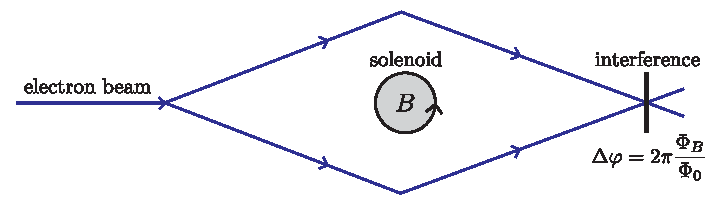
\includegraphics[]{Figures/Chapter7/aharonov_bohm.pdf}
\caption[The Aharonov-Bohm experiment]{The Aharonov-Bohm experiment. A coherent electron beam is split into two paths surrounding a solenoid which produces a non-zero magnetic field $\mathbf{B}$ inside the gray region and $\mathbf{B}=0$ outside. The two beams are later recombined and an interference pastern reveals a phase difference $\Delta\varphi = 2\pi \Phi_B/\Phi_0$ equal to the magnetic flux enclosed by the electron's path.}
\label{fig:aharonov_bohm}
\end{center}
\end{figure*}

This Aharonov-Bohm phase can be interpreted as an example of a Berry phase in real space. For a charged particle in the presence of a vector potential the momentum dependence of the free-particle Hamiltonian is modified $\mathbf{p}\rightarrow\mathbf{p}-q\mathbf{A}$ so that the wave function will depend on the magnetic vector potential as well. Using Equations~\ref{eq:berry_phase} and~\ref{eq:berry_connection} it can be shown that the Berry phase associated to a closed path around the solenoid is exactly equal to the Aharonov-Bohm phase: 
%
\begin{align}
	\gamma_n(\mathcal{C})=&\frac{e}{\hbar}\oint_{\mathcal{C}}\mathbf{A}(\mathbf{r})\cdot d\mathbf{r} \nonumber \\
	=& \frac{e}{\hbar}\int_{\mathcal{S}}\nabla\times\mathbf{A}\cdot d\mathbf{S} \nonumber \\
	=& \frac{e\Phi_B}{\hbar},
	\label{eq:aharonov_bohm_phase}
\end{align}

For this particular example, the Berry connection is exactly equal to the magnetic vector potential and the Berry curvature is the magnetic field. This gives us a very physical intuition for interpreting the Berry phase in terms of the `magnetic flux' from abstract sources of `magnetic fields' in parameter space.  

\subsection{Chern number}

The Chern number is conventionally used to describe the topology of materials which have an underlying crystalline structure. According to Bloch's theorem, the wave functions of a space periodic Hamiltonian can be written as $\ket{\psi(\k)}=e^{i\k\cdot\mathbf{r}}\ket{u(\k)}$, where $\ket{u(\k)}$ are periodic wave functions. If we define the Bloch Hamiltonian
%
\begin{equation}
	\hat{H}(\k)=e^{i\k\cdot\mathbf{r}}\hat{H}(\mathbf{r})e^{-i\k\cdot\mathbf{r}}, 
\end{equation}
%
their eigenvectors are given by $\ket{u(\k)}$ and the eigenvalues define the band structure. Translational symmetry implies that $\hat{H}(\k+\mathbf{a})=\hat{H}(\k)$ where $\mathbf{a}$ is a reciprocal lattice vector. The crystal momentum or quasimomentum is only defined within the periodic Brillouin zone and therefore can be mapped into a torus in $d$ dimensions if we glue the edges together.  

The Chern number of the $n$th band is defined as
%
\begin{equation}
	C_n=\frac{1}{2\pi}\int_{BZ}\mathbf{\Omega}_n d\k,
	\label{eq:chern_number}
\end{equation}
%
where the relevant parameter space is crystal momentum and the surface of integration corresponds to the BZ (a torus). The definition of Chern number is closely related to the definition of the Berry phase from Equation~\ref{eq:berry_connection}. For our previous example of a quantum Hall system, the integer proportionality factor in the quantized conductance is exactly equal to the Chern number. 

Just like two-dimensional surfaces are classified by the integral of their Gaussian curvature, the topology of Bloch bands and of quantum systems in general is determined by the integral of the Berry curvature. In a similar way, the integral connects local properties of a quantum system, the Berry connection, with a global topological invariant, the Chern number. One subtle difference is that the Euler characteristic is only determined by the surface (and its intrinsic Gaussian curvature) while the Chern number is defined both by a surface (the BZ) and an additional local curvature (the Berry curvature). By studying different Hamiltonians one can obtain a different Berry curvature, but the geometry of the BZ and thereby the surface of integration is typically defined by a torus\footnote{In next chapter we consider a case where this breaks down.}. This difference will be important later on when we describe the experiments performed to study a system with Rashba spin-orbit coupling and an unconventional topology. %Using our intuition from the Aharonov-Bohm phase, the Chern number can also be interpreted as the total flux from a `Berry field'  defined in the BZ and whose sources are `monopoles' given by degeneracies in the Hamiltonian. 

% Even though the Chern invariant was initially conceived to classify the topology of systems in momentum space, there have been experiments that studied the topology of quantum systems in other abstract parameter spaces, see for example ~\cite{roushan_observation_2014} and \cite{sugawa_second_2018}.

\section{The bulk-edge correspondence principle}

Earlier I mentioned that topological systems provide very robust channels for transporting things like electrical current and light. This transport phenomena typically arises when there is a spatial interface between two topologically distinct phases. The electrons skipping orbits at the interface of a (topological) quantum Hall material and (trivial) vacuum are one example of this. Notice that for this particular example the modes propagate along a given direction, they are chiral. In general one can expect to have modes moving along two directions, and the difference between the number of these modes $N_L - N_R$ is fixed and determined by the topology of the bulk states. The bulk-edge correspondence principle relates the difference in the number of these modes with the bulk topology of the materials at the interface:
%
\begin{equation}
	\Delta C=N_R - N_L
\end{equation}
%
where $\Delta C$ is the difference of Chern number on the interface. 

\section{Example: two-level model}
\label{sec:2_level_topology}

Many of the concepts introduced in the previous section can be readily applied and understood using a two-level model
%
\begin{equation}
	\hat{H}(\mathbf{k})= \mathbf{h}(\mathbf{k})\cdot\hat{\boldsymbol{\sigma}}
	\label{eq:2D_Hamiltonian}
\end{equation}
%
where $\hat{\boldsymbol{\sigma}}=(\sigma_x, \sigma_y, \sigma_z)$ are the Pauli matrices and $\mathbf{h}(\mathbf{k})=(h_x(\k),h_y(\k), h_z(\k))$ are functions of $\k$. This model has been used to describe a number of physical systems like graphene~\cite{haldane_model_1988} and spin-orbit coupled systems~\cite{bychkov_oscillatory_1984,dresselhaus_spin-orbit_1955}. Let us now consider the simple case $h(\k)=\k$, for which $\nabla_{\k}\hat{H}=\boldsymbol{\sigma}$ and using Equation~\ref{eq:alternative_berry_con} it can be shown that
%
\begin{equation}
	\mathbf{\Omega}=-\frac{\mathbf{h}}{2h^3}
	\label{eq:monopole}
\end{equation}
%
which can be recognized as the field of a Dirac monopole~\cite{dirac_paul_adrien_maurice_quantised_1931} with charge $-1/2$. The degeneracy in the energies that gives rise to the monopole is known as a Dirac point as the energies in that vicinity resemble the dispersion of a massless Dirac particle. It follows from Equation~\ref{eq:monopole} that the Berry phase gained by moving in a closed path $\mathcal{C}$ is equal to the flux from the monopole in the surface enclosed by $\mathcal{C}$ as is shown in Figure~\ref{fig:solid_angle}. This connects nicely with our intuition from the Aharonov-Bohm effect. For a closed surface enclosing the Dirac point, the Chern number is an integer equal to 1. 
%
\begin{figure*}[htb]
\begin{center}
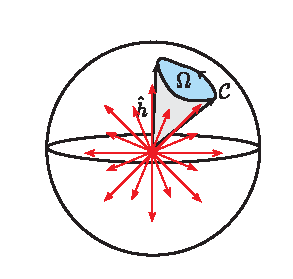
\includegraphics[]{Figures/Chapter7/solid_angle.pdf}
\caption[Graphical representation of Chern number]{For a two-level system, the Berry curvature from a Dirac point can be viewed as a Dirac monopole in momentum (parameter) space. The Chern number can be interpreted as the flux from the monopole on the solid angle subtended by the vector $\hat{h}(\k)$ or alternatively as the number of times $\hat{h}(\k)$ wraps around a unit sphere.}
\label{fig:solid_angle}
\end{center}
\end{figure*}

For a Hamiltonian with arbitrary $\mathbf{h}(\k)$ we can define a normalized vector $\hat{h}=\mathbf{h}/\vert\mathbf{h}\vert$ and the Chern number takes the form
%
\begin{equation}
	C=\frac{1}{4\pi}\int(\partial_{k_x}\hat{h}\times\partial_{k_y}\hat{h})\cdot\hat{h} \, d\k
\end{equation}
%
and can be interpreted as the number of times that the vector $\hat{h}(\k)$ wraps around a unit sphere~\cite{kaufmann_notes_2016}, a quantity that is known as the winding number.

% \note{My current points of confusion are the following:}
% Why is the Chern number for a single Dirac point on a torus a half? I'm thinking in particular for the quantum hall effect and the example on section 2 on the review on topological insulators. Also how to go from closed paths in parameter space to closed surface integrals?
% Also keep in mind Krammers theorem: for every energy eigenstate of a time-reversal symmetric system with half-integer total spin, there is at least one more eigenstate with the same energy. In other words, every energy level is at least doubly degenerate if it has half-integer spin.
% Why is $h_z\neq0$ the same as breaking time reversal symmetry? What about the other components? 

\section{Monopoles and Dirac strings}

We just gained some intuition about interpreting the Chern number as the flux from Dirac monopoles. But if we stick to our knowledge of electromagnetism we might remember that monopoles are forbidden since
%
\begin{equation}
	\int_{\mathcal{S}}\mathbf{B}\cdot d\mathbf{S}=\int_{V}(\nabla\cdot\mathbf{B})dV
\end{equation}
%
and $\nabla\cdot\mathbf{B}=\nabla\cdot(\nabla\times\mathbf{A})=0$. So how is this possible? The solution to this problem was envisioned by Dirac~\cite{dirac_paul_adrien_maurice_quantised_1931} and is now called a Dirac string. If we consider an semi-infinitely long and infinitesimally thin solenoid, the magnetic field in the finite end will resemble that of a monopole as can be seen in Figure~\ref{fig:monopole}. This tiny solenoid corresponds to the Dirac string. 
%
\begin{figure*}[htb]
\begin{center}
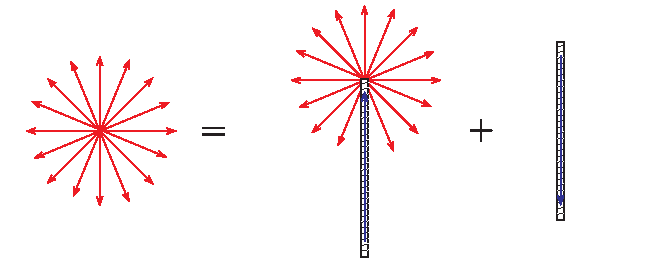
\includegraphics[]{Figures/Chapter7/monopole.pdf}
\caption[Graphical representation of Chern number]{For a two-level system, the Berry curvature from a Dirac point can be viewed as a Dirac monopole in momentum (parameter) space. The Chern number can be interpreted as the flux from the monopole on the solid angle subtended by the vector $\hat{h}(\k)$ or alternatively as the number of times $\hat{h}(\k)$ wraps around a unit sphere.}
\label{fig:monopole}
\end{center}
\end{figure*}
A more mathematical interpretation of these strings comes from the fact that the vector potential of a monopole has `lines' where it becomes singular. For example for a particular gauge we can write
%
\begin{equation}
	\mathbf{A}(\r)=g\frac{-y\ex+x\ey}{r(r+z)}
\end{equation}
%
which is singular for the negative $z$ axis where $z=-r$. The orientation of the Dirac string is gauge dependent, something that should not surprise or bother us at this point. However, the physical effects of the Dirac string should be gauge independent, or in other words, the Aharonov-Bohm phase gained by a charged particle moving in a path that encloses the string should be an integer multiple of $2\pi$. This is argument gives rise to the Dirac charge quantization~\cite{dirac_paul_adrien_maurice_quantised_1931}, and in the context of topology, it guarantees that when we calculate the Berry phase by integrating the Berry connection (vector field) along a path that enclose a Dirac string, its effect will be indistinguishable. 


% In order for the field resulting from this string to be indistinguishable from that of a monopole, the Aharonov-Bohm phase gained by an electron moving around it has to be indistinguishable. For a monopole with charge $g$ this means that $2\pi N=\Phi_g/\Phi_0$

% A For this gauge choice, the $-z$ axis corresponds to the Dirac string. The orientation of the string might change for a different basis but if we demand that the field resulting from either of this vector potentials 


% I mentioned earlier that the Berry curvature from a Dirac point looks like a monopole and that the flux from this monopole on a closed surface is equal to the Chern number. This 
% If we try to write the vector potential for a monopole we will find that there is a line where it becomes singular. For example, for a monopole with charge g we can write
% %
% \begin{equation}
% 	\mathbf{A}(\r)=g\frac{-y\ex+x\ey}{r(r+z)}
% \end{equation}
% %
% which is singular at the south pole where $z=-r$. We could alternatively write 
% %
% \begin{equation}
% 	\mathbf{A}(\r)=g\frac{y\ex-x\ey}{r(r-z)}
% \end{equation}
% %
% which leads to the same 
% The existence of Dirac monopoles comes with some interesting consequences. A magnetic monopole can be thought of as the end of a semi-infinitely long and infinitesimally thin magnetic solenoid. In order for the field of the solenoid to be indistinguishable from that of a monopole, the Aharonov-Bohm phase gained by an electron moving around it has to be indistinguishable. For a monopole with charge $g$ this means that $2\pi N=\Phi_g/\Phi_0$

% . This thin solenoid can in fact be identified with  


% The existence of Dirac monopoles means that there has to be a singularity in the vector potential. 


% to be a Dirac string~\cite{dirac_paul_adrien_maurice_quantised_1931}. Dirac envisioned having an infinitesimally thin solenoid whose end looks like a magnetic charge. The monopole can only be identified as such if the thin solenoid is not experimentally detectable.

% Lets imagine for a moment 
% %
% \begin{equation}
% 	\int_{\mathcal{S}}\mathbf{B}\cdot d\mathbf{S}=q_m
% \end{equation}

% It is possible to find a magnetic vector potential 
% m This objects were conceived by Dirac as tiny solenoids
% If magnetic monopoles exist then electric charge must be quantized
% In electromagnetic theory 

% A consequence of the Berry connection being singular 

% This vector potential has one problem. It is singular at the north pole (z = r). In fact, one can prove that no matter which gauge one uses, there will always be a singularity point.

% Degeneracies as sources of Berry curvature field. There must therefore be Dirac strings as well...

\section{Conclusions}

Topology plays a very important role both in math and in physics. In this Chapter I reviewed the basic concepts of topology in the context of condensed matter physics that will be relevant for our experiments with unconventional topology. As a closing remark, Figure~\ref{fig:topology_analogies} summarizes the main concepts that were introduced and is a reminder that topological invariants are global properties defined in terms of integrals of local properties. Furthermore, we can use our intuition from electromagnetic theory to interpret topological invariants in quantum mechanics. 

 \begin{figure*}[htb]
\begin{center}
\includegraphics[]{Figures/Chapter7/topology_analogies.pdf}
\caption[Different topological invariants]{The Euler characteristic and the Chern number are topological invariants defined by integrals of local curvatures. The Aharonov-Bohm phase gives us physical intuition to interpret the Chern number as the flux from a `Berry field'.}
\label{fig:topology_analogies}
\end{center}
\end{figure*}

%%%%%%%%%%%%%%%%%%%%%%%%%%%%%%%%%%%%%%%%%%%%%%%%%%%%%%%%%%%%%%%
%
%Graveyard
%
%%%%%%%%%%%%%%%%%%%%%%%%%%%%%%%%%%%%%%%%%%%%%%%%%%%%%%%%%%%%%%%%


% If there is inversion ($\mathcal{P}$) and time reversal ($\mathcal{T}$) symmetry $h_z(\k)=0$ and there are points where the Hamiltonian in Equation~\ref{eq:2D_Hamiltonian} becomes singular. For example, in graphene this occurs in two points. In the vicinity of these points $\q=\k-\k_0$, Equation~\ref{eq:2D_Hamiltonian} resembles the Hamiltonian of a massles Dirac fermion $\hat H(\mathbf k)=\hbar v_F\mathbf q\cdot \vec \sigma$, where $v_F$ is a velocity. 
 
% The $\mathcal{T}$ symmetry can be broken for example by applying a magnetic field, in which case the degeneracy at the Dirac point is broken and \ref{eq:2D_Hamiltonian} becomes a massive Dirac Hamiltonian. 


%  For simplicity lets consider $\mathbf{h}(\k)=h(\sin\theta\cos\phi,\sin\theta\sin\phi,\cos\theta)$. The Hamiltonian has eigenvalues $\pm h$ and the eigenstates are
% %
% \begin{align}
% 	\ket{+}=&(\sin\theta/2e^{-i\phi}, -\cos\theta/2 )  \nonumber \\
% 	\ket{-}=&(\cos\theta/2e^{-i\phi}, \sin\theta/2) 
% \end{align}
%

%For a small and constant value of $h_z$, $\hat{h}$ only wraps around the top or lower half of the Bloch sphere, depending on the sign of $h_z$.

% If $h_z=0$ there are Dirac points\footnote{This can happen if there is inversion ($\mathcal{P}$) and time reversal ($\mathcal{T}$) symmetry} where $\vert\mathbf{h}\vert=0$ and near these ponits Equation~\ref{eq:2D_Hamiltonian} locally resembles the Hamiltonian of a massless Dirac fermion. Near the Dirac points the Berry connection can be written as
